%acmsmall: The default journal template style.
%acmlarge: Used by JOCCH and TAP.
%acmtog: Used by TOG.
%acmconf: The default proceedings template style.
%sigchi: Used for SIGCHI conference articles.
%sigchi-a: Used for SIGCHI ``Extended Abstract'' articles.
%sigplan: Used for SIGPLAN conference articles.
\documentclass[format=acmtog, 12pt, screen=true, review=false]{acmart}

%% \BibTeX command to typeset BibTeX logo in the docs
\AtBeginDocument{%
  \providecommand\BibTeX{{%
    \normalfont B\kern-0.5em{\scshape i\kern-0.25em b}\kern-0.8em\TeX}}}

%% Rights management information.  This information is sent to you
%% when you complete the rights form.  These commands have SAMPLE
%% values in them; it is your responsibility as an author to replace
%% the commands and values with those provided to you when you
%% complete the rights form.
\setcopyright{acmcopyright}
\copyrightyear{2019}
\acmYear{2019}
\acmDOI{123456789}

%%
%% These commands are for a JOURNAL article.
\acmJournal{TOMACS}
\acmVolume{Vol}
\acmNumber{Num}
\acmArticle{Art}
\acmMonth{Month}

%%
%% Submission ID.
%% Use this when submitting an article to a sponsored event. You'll
%% receive a unique submission ID from the organizers
%% of the event, and this ID should be used as the parameter to this command.
\acmSubmissionID{123-456-789}

%%
%% The majority of ACM publications use numbered citations and
%% references.  The command \citestyle{authoryear} switches to the
%% "author year" style.
%% If you are preparing content for an event
%% sponsored by ACM SIGGRAPH, you must use the "author year" style of
%% citations and references.
%\citestyle{acmauthoryear}
\citestyle{acmnumeric}

%% Useful packages
\usepackage{multicol}
\usepackage[UKenglish]{babel}
\usepackage{comment}
\usepackage[T1]{fontenc}
\usepackage{enumitem}
\usepackage{graphicx}
\usepackage{textcomp}
\usepackage{amsmath}
\usepackage{booktabs}
\usepackage{tabu}
\usepackage{float}

%%
%% The "title" command has an optional parameter,
%% allowing the author to define a "short title" to be used in page headers.
\title[Dynamic Impact Response of LG]{Dynamic Impact Response of Laminated Window Glass}
\subtitle{Plan of Investigation}
%If your title is lengthy, you must define a short version to be used
%in the page headers, to prevent overlapping text. The \texttt{title}
%command has a ``short title'' parameter:

%%
%% The "author" command and its associated commands are used to define
%% the authors and their affiliations.
%% Of note is the shared affiliation of the first two authors, and the
%% "authornote" and "authornotemark" commands
%% used to denote shared contribution to the research.

%If your author list is lengthy, you must define a shortened version of
%the list of authors to be used in the page headers, to prevent
%overlapping text. The following command should be placed just after
%the last \texttt{\author{}} definition:
%\begin{verbatim}
%  \renewcommand{\shortauthors}{McCartney, et al.}
%\end{verbatim}
%Omitting this command will force the use of a concatenated list of all
%of the authors' names, which may result in overlapping text in the
%page headers.

\author{John-Paul Latham}
\authornote{Imperial College London.}
\email{j.p.latham@imperial.ac.uk}

\author{Jason Xiang}
\authornotemark[1]
\email{j.xiang@imperial.ac.uk}

\author{Ado Farsi}
\authornotemark[1]
\email{ado.farsi@imperial.ac.uk}

\author{Michael Trapp}
\email{mt5918@ic.ac.uk}
\orcid{1234-5678-9012}
\authornotemark[1]

%%
%% By default, the full list of authors will be used in the page
%% headers. Often, this list is too long, and will overlap
%% other information printed in the page headers. This command allows
%% the author to define a more concise list
%% of authors' names for this purpose.
\renewcommand{\shortauthors}{Latham et al.}

%% end of the preamble, start of the body of the document source.
\begin{document}

%%
%% The abstract is a short summary of the work to be presented in the
%% article.
\begin{abstract}
  Optimising the dynamic impact response of laminated window glass is important to improving public safety and security. Example applications involve counter-acting malicious human activity, persistance against natural hazards, and preventing and reducing the effects of injuries and accidents due to flying glass debris. A novel coupled multi-physics software has been developed further by the AMCG group at Imperial College. In the past, the software has been successfully applied to geological applications. In this project, the software is applied to numerically predict the dynamic impact response of laminated window glass. The objective is to accurately and realistically simulate the impact of a projectile on a laminated glass plate in 2D (3D). The model geometry is prepared and stored in text files. The results are visualised and validated using numerical experiments from other research.
\end{abstract}

%%
%% The code below is generated by the tool at http://dl.acm.org/ccs.cfm.
%% Please copy and paste the code instead of the example below.
%%
%\section{CCS Concepts and User-Defined Keywords}
%
%Two elements of the ``acmart'' document class provide powerful
%taxonomic tools for you to help readers find your work in an online
%search.
%
%The ACM Computing Classification System ---
%\url{https://www.acm.org/publications/class-2012} --- is a set of
%classifiers and concepts that describe the computing
%discipline. Authors can select entries from this classification
%system, via \url{https://dl.acm.org/ccs/ccs.cfm}, and generate the
%commands to be included in the \LaTeX\ source.
\begin{CCSXML}
<ccs2012>
<concept>
<concept_id>10010405.10010432.10010439</concept_id>
<concept_desc>Applied computing~Engineering</concept_desc>
<concept_significance>300</concept_significance>
</concept>
</ccs2012>
\end{CCSXML}
\ccsdesc[300]{Applied computing~Engineering}

%%
%% Keywords. The author(s) should pick words that accurately describe
%% the work being presented. Separate the keywords with commas.
\keywords{Laminated Window Glass, Impact Response, Fracturing, Numerical Modelling, FEMDEM, Combined Discrete-Finite Element Method, Coupled Physics Model, Multi-Phase Model, Brittle, Crack Initiation, Crack Propagation, Computational Modelling, ACMG, Imperial College}
%%
%% This command processes the author and affiliation and title
%% information and builds the first part of the formatted document.

\maketitle

\section{Introduction}
%A good introduction “sets the scene” for the reader. It starts with an overview of the project research area, moves on to the current state-of-play, and then ends with a statement of the aims and objectives of the project, and how you plan to achieve them. 

Laminated glass is a sandwich structure consisting of two glass plies and an adhered inter-layer (or inter-face). The task of the inter-layer is the absorption of impact energy and the maintenance of adhesion to the plies \cite{Wu14}. An optional back layer improves structural stability and additional energy absorption \cite{Bio10, Bra10}.

\bigbreak
Inter-layer materials include polymers such as traditional polyvinyl butyral (\texttt{PVB}), thermoplastic polyurethane (\texttt{TPU}), and most recently \texttt{SentryGlas}\textregistered Plus (\texttt{SGP}) \cite{Moh18, Wan18}. The back layer traditionally consists of polycarbonate (\texttt{PC}) \cite{Mon04, Bra10}.

\bigbreak
Advantageous properties of laminated glass include a relatively high penetration resistance, low weight \cite{Wu14} and the bonding of glass fragments to reduce the risk of injuries \cite{Che17, Flo98, Ji98}. 

\bigbreak
Breakage of the inner ply significantly reduces strength and facilitates a full collapse of the glass \cite{Flo98}. The predictions of crack initiation and propagation pose a significant challenge and requires additional research effort.

\section{Fracture Theory}

\subsection{Local Stress Concentration}

Breaking atomic bonds in brittle continuum media to form cracks requires the minimum assumed force

\begin{equation}
\label{eq:minforce}
    P = P_{\rm{C}}\,\rm{sin}\left(\frac{\pi x_{\rm{0}}}{\lambda}\right)\approx \frac{P_{\rm{C}}\pi x_{\rm{0}}}{\lambda}\,,
\end{equation}

where $P_C$ is the atom-dependent cohesive force and $\lambda$ is the distance from atom origin $x_0$. The stiffness yields

\begin{equation}
    k=\frac{P}{x_0}=\frac{P_{\rm{C}}\pi}{\lambda}\,.
\end{equation}

The cohesive strength of the material per unit bonds yields

\begin{equation}
\label{eq:cohesivestrength}
    \sigma_{\rm{C}}=E\varepsilon=\frac{E\lambda}{\pi x_{\rm{0}}} \,.
\end{equation}

The surface energy of the material, consisting of the energy of broken atomic bonds in the unit area, is given by

\begin{equation}
    \label{eq:surfaceenergy}
    \gamma_{\rm{S}}=\frac{1}{2}\int_{0}^{\lambda}\sigma_{\rm{C}}\,\rm{sin}\left(\frac{\pi x}{\lambda}\right)dx=\sigma_{\rm{C}}\frac{\lambda}{\pi} \,.
\end{equation}

Substituting eq. \ref{eq:cohesivestrength} into eq. \ref{eq:surfaceenergy} yields the cohesive strength

\begin{equation}
    \label{eq:newcohesivestrength}
    \sigma_{\rm{C}}=\sqrt{\frac{E}{\gamma_{\rm{S}}\,x_{\rm{0}}}}\,.
\end{equation}

Applying $\sigma_{\rm{C}}$ on an infinite plate containing an elliptical hole ($2a \times 2b$) generates vertex stress

\begin{equation}
\label{eq:vertexstress}
    \sigma_{\rm{V}}=\sigma_{\rm{C}}\left(1+\frac{2a}{b}\right)=\sigma_{\rm{C}}\left(1+2\sqrt{\frac{a}{\rho}}\right)\,,
\end{equation}

with curvature $\rho=b^2/a$ and stress concentration $k_{\rm{t}} = \sigma_{\rm{V}} / \sigma_{\rm{C}}$ \cite{And05}. Substituting eq. \ref{eq:newcohesivestrength} into \ref{eq:vertexstress} yields the minimum stress to create fracturing 

\begin{equation}
    \label{eq:FailureStressLocalStress}
    \sigma_{\rm{f}}=\sqrt{\frac{E\gamma_{\rm{S}}}{4a}} \,.
\end{equation}

Eq. \ref{eq:FailureStressLocalStress} is based on a continuum assumption and not valid on atomic level and is only an approximation of reality. Local stress intensification is provided by pre-existing micro-structural material flaws (inhomogeneities, discontinuities) such as micro-cracks and voids \cite{Sch12}. Application of stress $\sigma_{\rm{f}}$ causes these flaws to grow in size. \cite{Flo98, Pel16}. Critical flaws, causing complete structural failure, are usually found on the cut and machined glass edges \cite{Pel16}.

\subsection{Energy balance}

According to global energy balance models by Irwin and Griffith \cite{Sch12, And05}, crack area extension $dA$ requires a sufficiently large potential energy $\Pi$ (the energy release rate $G$) to overcome the surface energy $W_{\rm{S}}$ (the material resistance or crack resistance $R$). The rate of change of total energy is given by

\begin{equation}
    \label{eq:EnergyBalance}
    \frac{\rm{d}E_{\rm{t}}}{\rm{d}A}=G+R=\frac{\rm{d}\Pi}{\rm{d}A}+\frac{\rm{d}W_{\rm{S}}}{\rm{d}A}\geq0\,,
\end{equation}

Equality in eq. \ref{eq:EnergyBalance} results in stable crack growth, inequality in unstable growth. Applying the criterion for an infinite plate with a crack of length $a$ yields

\begin{equation}
\frac{\rm{d}E_{\rm{t}}}{\rm{d}A}=-\frac{\pi\sigma^2a}{E}+2\gamma_S\leq0\,,
\end{equation}

where $\sigma$ is the applied stress. Hence the minimum stress to generate fracturing is given by

\begin{equation}
    \label{eq:FailureStressEnergyBalance}
    \sigma_{\rm{f}} = \sqrt{\frac{2E\gamma_{\rm{S}}}{\pi a}}\,.
\end{equation}

For sharp cracks ($a>>$) in brittle materials, eq. \ref{eq:FailureStressLocalStress} and eq. \ref{eq:FailureStressEnergyBalance} are consistent. Kuruvita et al. \cite{Kur14} developed their own energy balance model.

\subsection{Stress Intensity Factor}

Loading at a crack is subdivided into three categories. Mode I refers to principal loading perpendicular to the crack plane, Mode II refers to in-plane shear and Mode III to out-of-plane shear. The stress field of a linear elastic cracked body is approximated by

\begin{equation}
    \sigma_{\rm{ij}}=\frac{K}{\sqrt{2\pi r}}f_{\rm{ij}}(\theta)\,,
\end{equation}

with distance $r$ and angle $\theta$ from the crack tip, dimensionless function $f_{\rm{ij}}(\theta)$ and stress intensity factor $K=\{K_{\rm{I}},K_{\rm{II}},K_{\rm{III}}\}$. The definitions of the dimensionless angular functions are listed in the appendix. The stress intensity factors \cite{And05, Xu11} are derived empirically. Uniform tensile stress applied on an infinite plane (\textt{Young's Modulus} $E$) with a through crack generates energy release rate

\begin{equation}
    G = \frac{K_{\rm{I}}^2}{E}\,\,.
\end{equation}

\subsection{Combined Single and Smeared Crack Model}

Smeared crack model describe cracks locally via non-linear constitutive laws. The Dougale model is a common  

\begin{figure}[h]
  \centering
  \label{fig:Douglas}
  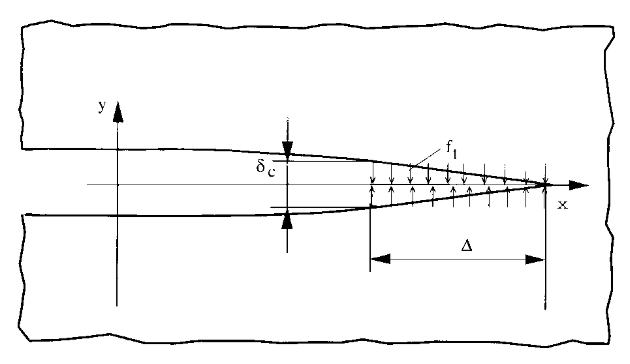
\includegraphics[width=\linewidth]{Dougale.PNG}
  \caption{Dougale Model \cite{Lat15}}
  %\Description{Dougale Model \cite{Lat15}}
\end{figure}

The Dugdale model is a relatively simple non-linear model for a crack with a plastic zone at its tips, where the zone of plastically strained material is replaced by a zone of weakened bonds between the crack walls, Figure 1. As the crack walls separate the bond stress reaches maximum ft. At the point when the separation reaches critical value ?=?c the bonding stress drops to zero.


\bigbreak
The normal stress σ and the shear stress τ, corresponding to the normal displacement δn and the shear displacement δs between triangular surfaces, respectively, are calculated according to a constitutive law as shown above. The peak stress f on this stress-displacement curve represents the material strength, so for normal stress σ, it means tensile strength ft; and for shear stress τ, it means shear strength fs. The tensile strength ft is assumed to be a constant, while the shear strength fs is defined by the Mohr-Coulomb criterion with a tension cut-off where c is cohesion,  ϕ is internal friction angle, σn is the normal stress acting perpendicular to the shear direction. Note here the engineering mechanics sign convention is used, so tensile stress is positive and compressive stress is negative. δp is the maximum elastic displacement corresponding to peak stress f between two triangular surfaces in a joint element, and δc is the critical displacement, at which the joint element fails.

For a single mode I tensile fracture, for example, the physical meanings of δp and δc is illustrated below. For this case, because it is pure tension, δp is represented by δnp and δc is represented by δnc. In the below figure, the white area represents the continuum domain that is intact without any fractures; the light yellow area represents physically discrete fracture; the orange area between them is defined as plastic zone, which corresponds to the strain softening part (δnp ~ δnc) in the above figure. It is worth noting that in the figure below, which represents the crack propagating from right to left, the short vertical red bars between the red line and the blue line represent the magnitudes of normal stress σ in the joint elements. It can be seen that δnp represents the position, where the normal stress σ in the joint element reaches its peak value (tensile strength ft); ahead of this position (to the discrete fracture direction), the domain is at a strain softening stage (orange area), which means the normal stress σ decreases from tensile strength ft to zero while the normal displacements δn increases from δnp to δnc. After this moment (when δn = δnc), this joint element will fail and the constitutive law is not applied to this failed joint element anymore. Instead, the interaction between the fracture walls will be counted as contact force, including normal compression and sliding friction, which is calculated by the contact algorithms. 

\begin{enumerate}
    \item Contact Algorithm \cite{Mun}
\end{enumerate}

The detailed contact algorithms for the three-dimensional FEMDEM method can be found in Munjiza’s book (2004). Furthermore, empirical microscale roughness effects can also be introduced via a Joint Constitutive Model, to account for dilation and normal stiffness on stressed new and pre-existing fracture surfaces, for implementation of empirical JCM, see Lei et al. (in review, 2016).

Munjiza et al. \cite{Mun99} applies a combined single and smeared crack model. 

\subsection{Different Analytical Models}

Mili et al. \cite{Mil12} attempted application of the \texttt{Hertzian Contact Law}, but only found accurate predictions for low impact velocities. Kuruvita et al. \cite{Kur14} investigated a spring-mass model and a wave propagation method for infinitely thick plates. Pel et al.The Rankine fracture criterion predicts crack initiation after the maximum principal stress reaches the material strength \cite{Pel16}.

\section{Background Research}

%t should also contain a BACKGROUND RESEARCH section. This might include a survey of relevant literature, programming methods or techniques, as well as any relevant discussion on different options that were available to you and a justification for any decisions that you will have made. 

%If a key part of your project is the development of a software product, then you will need to include sections describing the software engineering method that you followed and detailing the results obtained during the different development phases such as requirements analysis, design, implementation and testing.  

%If your project is mostly theoretical, then you should include sections detailing the development of your theory. This might include small programs to investigate certain aspects, explanations of algorithms, or descriptions of any particularly hard bits of theory. A theoretical project will probably have a section on results and some sections on their analysis. 

%If your project involves computational experiments with real-world data, you will need a section or sections on experimental results, analysis, and conclusions derived from the experiments.

\subsection{Experimental Studies}

Relevant parameters of the impact projectile include the normal velocity \cite{Gra98, Kur14, Dar13, Wu14}, the mass \cite{Kur14, Dar13}, the angle \cite{Gra98, Kur14, Dar13}, the shape \cite{Dar13} and the size \cite{Wu14}.

\bigbreak
Relevant parameters for the outer glass ply include its dimensions \cite{Wan18}, its mass, the support conditions \cite{Wan18} and the make-up \cite{Wan18}.

\bigbreak
For the inter-layer, the material \cite{Moh18, Wan18, Mon04}, thickness \cite{Ji98, Kur14, Wan18} and temperature \cite{Moh18, Zha19} are relevant.

\bigbreak
Dynamic impact on laminated glass comprises hard and soft body impact \cite{Moh17}. Hard body impact such as ballistic impact \cite{Bra10} causes minimal deformation to the projectile, while soft body impact such as bird impact \cite{Moh17} causes the projectile to undergo extensive deformation.

\bigbreak
Low velocity ($\approx 20\,\mathrm{m}/\mathrm{s}$) hard impact experiments include the use of projectiles in form of road construction chippings \cite{Gra98}, ballistics \cite{Mon04}, drop-down weights \cite{Che15, Mil12, Wan18}, aluminum projectiles \cite{Mil12} and steel balls \cite{Beh99, Flo98, Wan18}. High velocity (around $180 m/s$) soft impact experiments include the use of silicon rubber projectiles \cite{Moh17} and gas guns \cite{Moh18}.

\bigbreak
Xu et al. \cite{Xu11} and Gao et al. \cite{Gao14} numerically carried out quasi-static and dynamic \texttt{Split Hopkinson Pressure Bar} (\texttt{SHPB}) compression experiments under different strain/loading rates. 

\bigbreak
Wang et al. \cite{Wan18} found that the panel size had an inferior effect on the breakage resistance \cite{Wan18}. Similarly, Monteleone et al. \cite{Mon04} found that only a local area of the ply around the impact absorbed the impact energy for high velocities.

\bigbreak
Kuruvita et al. \cite{Kur14} found that impact velocity and plate thickness contributed significantly towards the impact resistance, compared to impact mass and inter-layer thickness. Wang et al. \cite{Wan18} found an increased inter-layer thickness to have a negative effect on energy absorption. Liu et al. \cite{Liu16} established that the inter-layer thickness did not contribute towards energy absorption. In contrast, Behr and Kremer \cite{Beh99} found an increased inter-layer thickness to better protect the inner ply. Kim et al. \cite{Kim16} numerically optimised the \texttt{PVB} inter-layer constitution to prevent all damage to the inner glass ply.

\bigbreak
Liu et al. \cite{Liu16} numerically investigated the optimisability of the inter-layer in terms energy absorption by simulating the impact of a human head. Zhang et al. \cite{Zha19} investigated the influence of temperature on the inter-layer and found that a hybrid \texttt{TPU}/\texttt{SGP}/\texttt{TPU} inter-layer performed best over the entire range of tested temperatures.

%%%%%%%%%%%%%%%%%%%%%%%%%%%%%%%%%%%%%%%%%%%%%%%%%%%%%%%%%%%%%%%%%%%%%%%%%%%%%%%%%%%%%%%%%%%%%%%%
%%%%%%%%%%%%%%%%%%%%%%%%%%%%%%%%%%%%%%%%%%%%%%%%%%%%%%%%%%%%%%%%%%%%%%%%%%%%%%%%%%%%%%%%%%%%%%%%
%%%%%%%%%%%%%%%%%%%%%%%%%%%%%%%%%%%%%%%%%%%%%%%%%%%%%%%%%%%%%%%%%%%%%%%%%%%%%%%%%%%%%%%%%%%%%%%%
%%%%%%%%%%%%%%%%%%%%%%%%%%%%%%%%%%%%%%%%%%%%%%%%%%%%%%%%%%%%%%%%%%%%%%%%%%%%%%%%%%%%%%%%%%%%%%%%

\subsection{Numerical Simulations}

%Motivation
The task of fracture models is to predict crack initiation and propagation. Classical fracture models, e.g. maximum principal stress and strain \cite{Alt17}, cannot predict crack initiation and propagation sufficiently accurate in most situations. 

\bigbreak
%FEM and DEM
Hence numerical finite element simulations have been conducted by various authors using commercial software such as \texttt{DYNA2D}, \texttt{LS-DYNA3D} and \texttt{ABAQUS}. A disadvantage of pure FEM methods is the inefficient solid-gas coupling and high computational costs. Discrete element methods (\texttt{DEM}) treat each fracture as a seperate body, but are not able to accurately model the common cracking pattern of glass \cite{Che17}.

\bigbreak
%FEMDEM
In contrast, the combined discrete finite element method \texttt{FEMDEM} \cite{Wan18, Mun95, Mun99, Mun04, Mun12, Mun13, Guo16, Gao14, Xu14, Che18} is able to model both deformation and interaction of matrix bodies. The discrete elements consist of clusters of deformable finite elements. Cracks propagate along common finite element boundaries. The method remedyingly combines the solid interface and fracturing. Fracturing results in the formation of new discrete elements \cite{Mun13}. The driving equations of motion are given by

\begin{equation}
    M\ddot{x}+\mu\dot{x}+f_{int}=f_{ext}=f_{\rm{l}}+f_{\rm{b}}+f_{\rm{c}}\,,
\end{equation}

with lumped nodal mass matrix $M$, nodal displacements $x$, viscosity $\mu$, internal nodal forces $f_{\rm{int}}$ and external nodal forces $f_{\rm{ext}}$. External forces contain consist of external loads $f_{\rm{l}}$, bonding forces $f_{\rm{b}}$ and contact forces $f_{\rm{c}}$. Internal forces $f_{\rm{int}}$ are generated by element deformation. FEMDEM systems solve these equations via explicit
time integration using the forward Euler method \cite{Lei16}.

\bigbreak
%Munjiza
The combination of discrete and finite elements is established via an interaction algorithm \cite{Lei16}, which is based on the original distributed potential contact force approach \cite{Mun13}. The contact forces between a contractor and target solid are given by

\begin{equation}
    f_c=\int_{\Gamma_{\rm{c}}}n\left(\varphi_{\rm{c}}-\varphi_{\rm{t}}\rm{d}\Gamma_{\rm{c}}\right)\,,
\end{equation}

with outward unit normal n to penetration boundary $\Gamma_{\rm{c}}$, and potential functions $\varphi_{\rm{c}}$ and $\varphi_{\rm{t}}$ for contractor and target. The contractor applies to the target a normal contact force

\begin{equation}
    f_n=-n\int_0^{L_{\rm{p}}} p\varphi(l){\rm{d}}l\,,
\end{equation}

with penetration length $L_{\rm{p}}$, potential function $\varphi$ along the target edge and penalty term $p$. It also applies a tangential friction force 

\begin{equation}
    f_{\rm{t}}=\mu_{mob}\lVert f_{\rm{n}} \rVert\frac{\varv_{\rm{r}}}{\lVert \varv_{\rm{r}}\rVert}\,,
\end{equation}

with relative velocity $v_{\rm{r}}$ at the Gauss point and mobilised friction coefficient $\mu_{mob}$, which varies during the shearing process.

\bigbreak
Conventional \texttt{FEMDEM} methods are significantly inaccurate, as their applied complex shaped polygons require deformability restriction constraints (so-called locking) to maintain stability of the simulation \cite{Lat15}. Munjiza et al. \cite{Mun13} developed a novel \texttt{2D} \texttt{FEMDEM} code, \texttt{Y}. The code is based on the so-called \texttt{F-bar} approach which uses 10-noded quadratic elements to reduce volumetric locking. Xiang et al. \cite{Xia09} developed the \texttt{Y}-code further and extended to \texttt{3D}. The novel \texttt{3D} \texttt{FEMDEM} code \texttt{Solidity}, \texttt{Y3D}, features coupled multi-body interaction \cite{Lat15}.
%%%%%%%%%%%%%%%%%%%%%%%%%%%%%%%%%%%%%%%%%%%%%%%%%%%%%%%%%%%%%%%%%%%%%%%%%%%%%%%%%%%%%%%%%%%%%%%%
%%%%%%%%%%%%%%%%%%%%%%%%%%%%%%%%%%%%%%%%%%%%%%%%%%%%%%%%%%%%%%%%%%%%%%%%%%%%%%%%%%%%%%%%%%%%%%%%
%%%%%%%%%%%%%%%%%%%%%%%%%%%%%%%%%%%%%%%%%%%%%%%%%%%%%%%%%%%%%%%%%%%%%%%%%%%%%%%%%%%%%%%%%%%%%%%%
%%%%%%%%%%%%%%%%%%%%%%%%%%%%%%%%%%%%%%%%%%%%%%%%%%%%%%%%%%%%%%%%%%%%%%%%%%%%%%%%%%%%%%%%%%%%%%%%

\section{Proposed Approach}

The approach is ... \\

Useful parameters are ...
\begin{enumerate}
    \item Timestep: $\Delta t:\,0.2\rm{nm}$ \cite{Che18}
    \item Glass layer: Triangular Mesh \cite{Che18}
    \item Glass layer: number of elements $=9180$ \cite{Che18}
    \item Glass layer: far field elemenet size $=2\rm{mm}$ \cite{Che18}
    \item Inter-layer: no thermal effects \cite{Che18}
    \item Inter-layer: purely elastic \cite{Che18, Ji98}
    \item Inter-layer: hyper-elastic \texttt{Mooney-Rivling} \cite{Che16}
    \item Inter-layer: linear visco-elastic \cite{Flo98}
    \item Inter-layer: \texttt{Mindlin Plate Theory} \cite{Yua17, ElS18}
    \item Inter-layer: visco-plastic \texttt{Johnson}-\texttt{Cook} \cite{Xu11, Gao14}
\end{enumerate}

\section{Milestones}

Planning Phase: 01 June - 28 June 2019
\begin{enumerate}
    \item Background Research
    \item Requirements Analysis
    \item Plan of Investigation
\end{enumerate}

Computation Phase: 29 June - 30 August 2019
\begin{enumerate}[resume]
    \item Set up Simulation
    \item Validate Parameters
    \item Tweak Parameters
    \item Finalize Report
\end{enumerate}

Presentation Phase: 31 August - early September 2019
\begin{enumerate}[resume]
    \item Oral presentation 
\end{enumerate}

\bibliographystyle{ACM-Reference-Format}
\setlength{\bibsep}{5.0pt}
\bibliography{LGP}

\appendix

\section{Mesh-Bound Numerical Fracture Models}

\subsection{EDM}
The element deletion method (\texttt{EDM}) or element erosion method (\texttt{EEM}) models crack initiation and propagation by either resetting the global mass matrix or by removing the element stresses \cite{Wan18, Liu16, Pel16}. Element removal equates to energy removal from the system, causing impact energy under-prediction \cite{Alt17, Ved17} - or fracture energy over-prediction \cite{Pel16} - and conflict with conservation laws \cite{Pel16}. Other drawbacks include inflexibility due to mesh-dependency and occasional instabilities \cite{Pel16}.

\subsection{CZM}

Another approach is the application of intrinsic and extrinsic \texttt{Cohesive Zone Models} (\texttt{CZM}), also called \texttt{Cohesive Crack Model} \cite{Gao14}. Such models involve adaptively inserting cohesive elements into the common boundaries between elements. This insertion creates an artificial compliance, i.e. an undesired elastic response. Compared to intrinsic models, extrinsic models additionally counter-act this response using formulated interface constraints via the Discontinuous Galerkin (\texttt{DG}) method. A disadvantage of the \texttt{DG} method is the significantly increased computational costs \cite{Wan18, Liu16, Che16}. Chen et al. \cite{Che16} modelled laminated glass using brick elements and applied an intrinsic cohesive formulation to model the adhesion between glass and \texttt{PVB}. 

\subsection{XFEM}

The extended finite element method (\texttt{XFEM}) \cite{Alt17, Xu10, Xu16} combines discontinuous and near-tip asymptotic fields through a unity method. \cite{Mun13} Although crack paths can be arbitrary, the explicit representation of the crack surface is required \cite{Rab04}. 

\bigbreak
The phantom-node method (\texttt{PNM}) \cite{VuB13} is an improved step-enriched XFEM method. In the standard phantom-node method (\texttt{PNM}), additional nodes, so-called phantom nodes, are defined along the crack, and the cracked element is replaced by two new elements. In contrast to XFEM, this new element handles the crack kinematics instead of the underlying element.

\subsection{BEM}

Another approach is the boundary element method (\texttt{BEM}) \cite{Mun13}.
%no clue what this is...
\section{Mesh-Free Numerical Fracture Models}

\subsection{SPH}

Smooth particle hydrodynamics (\texttt{SPH}) \cite{Moh17, Moh18} methods redefine the influence particles \cite{Mun13}.

\subsection{EFG}

Element-free Galerkin method (\texttt{EFG}) or Cracking Particle Method (\texttt{CPM})  \cite{Pel16, Fle96, Rab04, Rab07, Rab10}
define additional test and trial functions locally at the crack. The crack can be arbitrarily oriented, as its growth is represented discretely by activation of crack surfaces at individual particles. The crack is modelled by a local enrichment of the test and trial functions with a sign function (a variant of the Heaviside step function), so that the discontinuities are along the direction of the crack. The discontinuity consists of cylindrical planes centred at the particles in three dimensions, lines centred at the particles in two dimensions. The model is applied to several 2D problems and compared to experimental data. A shortcoming of this method is the required surface representation of the crack \cite{Rab04}.

\section{Angular Functions for Stress Field Ahead of Crack Tip}

\begin{align*}
    f_{\rm{xx}}^{\rm{I}}&=\rm{cos}\left(\frac{\theta}{2}\right)\left(1-\rm{sin}\left(\frac{\theta}{2}\right)\rm{sin}\left(\frac{3\theta}{2}\right)\right)\\
    f_{\rm{yy}}^{\rm{I}}&=\rm{cos}\left(\frac{\theta}{2}\right)\left(1+\rm{sin}\left(\frac{\theta}{2}\right)\rm{sin}\left(\frac{3\theta}{2}\right)\right)\\
    f_{\rm{xy}}^{\rm{I}}&=\rm{cos}\left(\frac{\theta}{2}\right)\rm{sin}\left(\frac{\theta}{2}\right)\rm{cos}\left(\frac{3\theta}{2}\right)\\
    \\
    f_{\rm{xx}}^{\rm{II}}&=-\rm{sin}\left(\frac{\theta}{2}\right)\left(2+\rm{cos}\left(\frac{\theta}{2}\right)\rm{cos}\left(\frac{3\theta}{2}\right)\right)\\
    f_{\rm{yy}}^{\rm{II}}&=\rm{sin}\left(\frac{\theta}{2}\right)\rm{cos}\left(\frac{\theta}{2}\right)\rm{cos}\left(\frac{3\theta}{2}\right)\\
    f_{\rm{xy}}^{\rm{II}}&=\rm{cos}\left(\frac{\theta}{2}\right)\left(1-\rm{sin}\left(\frac{\theta}{2}\right)\rm{sin}\left(\frac{3\theta}{2}\right)\right)\\
    \\
    f_{\rm{xz}}^{\rm{III}}&=-\rm{sin}\left(\frac{\theta}{2}\right)\\
    f_{\rm{yz}}^{\rm{III}}&=\rm{cos}\left(\frac{\theta}{2}\right)\\
\end{align*}

\end{document}


% Tables, Figures and Equations

%%%%%%%%%%%%%%%%%%%%%%%%%%%%%%%%%%%%%%%%%%%%%%%%%
%TABLES%
%%%%%%%%%%%%%%%%%%%%%%%%%%%%%%%%%%%%%%%%%%%%%%%%%
%\section{Tables}
%
%The ``\texttt{acmart}'' document class includes the ``\texttt{booktabs}''
%package --- \url{https://ctan.org/pkg/booktabs} --- for preparing
%high-quality tables.
%
%Table captions are placed {\itshape above} the table.
%
%Because tables cannot be split across pages, the best placement for
%them is typically the top of the page nearest their initial cite.  To
%ensure this proper ``floating'' placement of tables, use the
%environment \textbf{table} to enclose the table's contents and the
%table caption.  The contents of the table itself must go in the
%\textbf{tabular} environment, to be aligned properly in rows and
%columns, with the desired horizontal and vertical rules.  Again,
%detailed instructions on \textbf{tabular} material are found in the
%\textit{\LaTeX\ User's Guide}.
%
%Immediately following this sentence is the point at which
%Table~\ref{tab:freq} is included in the input file; compare the
%placement of the table here with the table in the printed output of
%this document.
%
%\begin{table}
%  \caption{Frequency of Special Characters}
%  \label{tab:freq}
%  \begin{tabular}{ccl}
%    \toprule
%    Non-English or Math&Frequency&Comments\\
%    \midrule
%    \O & 1 in 1,000& For Swedish names\\
%    $\pi$ & 1 in 5& Common in math\\
%    \$ & 4 in 5 & Used in business\\
%    $\Psi^2_1$ & 1 in 40,000& Unexplained usage\\
%  \bottomrule
%\end{tabular}
%\end{table}
%
%To set a wider table, which takes up the whole width of the page's
%live area, use the environment \textbf{table*} to enclose the table's
%contents and the table caption.  As with a single-column table, this
%wide table will ``float'' to a location deemed more
%desirable. Immediately following this sentence is the point at which
%Table~\ref{tab:commands} is included in the input file; again, it is
%instructive to compare the placement of the table here with the table
%in the printed output of this document.
%
%\begin{table*}
%  \caption{Some Typical Commands}
%  \label{tab:commands}
%  \begin{tabular}{ccl}
%    \toprule
%    Command &A Number & Comments\\
%    \midrule
%    \texttt{{\char'134}author} & 100& Author \\
%    \texttt{{\char'134}table}& 300 & For tables\\
%    \texttt{{\char'134}table*}& 400& For wider tables\\
%    \bottomrule
%  \end{tabular}
%\end{table*}
%
%%%%%%%%%%%%%%%%%%%%%%%%%%%%%%%%%%%%%%%%%%%%%%%%%
%%%%%%%%%%%%%%%%%%%%%%%%%%%%%%%%%%%%%%%%%%%%%%%%%
%%%%%%%%%%%%%%%%%%%%%%%%%%%%%%%%%%%%%%%%%%%%%%%%%
%Equations%
%%%%%%%%%%%%%%%%%%%%%%%%%%%%%%%%%%%%%%%%%%%%%%%%%
%\section{Math Equations}
%You may want to display math equations in three distinct styles:
%inline, numbered or non-numbered display.  Each of the three are
%discussed in the next sections.
%
%\subsection{Inline (In-text) Equations}
%A formula that appears in the running text is called an inline or
%in-text formula.  It is produced by the \textbf{math} environment,
%which can be invoked with the usual
%\texttt{{\char'134}begin\,\ldots{\char'134}end} construction or with
%the short form \texttt{\$\,\ldots\$}. You can use any of the symbols
%and structures, from $\alpha$ to $\omega$, available in
%\LaTeX~\cite{Lamport:LaTeX}; this section will simply show a few
%examples of in-text equations in context. Notice how this equation:
%\begin{math}
%  \lim_{n\rightarrow \infty}x=0
%\end{math},
%set here in in-line math style, looks slightly different when
%set in display style.  (See next section).
%\subsection{Display Equations}
%A numbered display equation---one set off by vertical space from the
%text and centered horizontally---is produced by the \textbf{equation}
%environment. An unnumbered display equation is produced by the
%\textbf{displaymath} environment.
%Again, in either environment, you can use any of the symbols and
%structures available in \LaTeX\@; this section will just give a couple
%of examples of display equations in context.  First, consider the
%equation, shown as an inline equation above:
%\begin{equation}
%  \lim_{n\rightarrow \infty}x=0
%\end{equation}
%Notice how it is formatted somewhat differently in
%the \textbf{displaymath}
%environment.  Now, we'll enter an unnumbered equation:
%\begin{displaymath}
%  \sum_{i=0}^{\infty} x + 1
%\end{displaymath}
%and follow it with another numbered equation:
%\begin{equation}
%  \sum_{i=0}^{\infty}x_i=\int_{0}^{\pi+2} f
%\end{equation}
%just to demonstrate \LaTeX's able handling of numbering.
%%%%%%%%%%%%%%%%%%%%%%%%%%%%%%%%%%%%%%%%%%%%%%%%%
%%%%%%%%%%%%%%%%%%%%%%%%%%%%%%%%%%%%%%%%%%%%%%%%%
%%%%%%%%%%%%%%%%%%%%%%%%%%%%%%%%%%%%%%%%%%%%%%%%%
%Figures%
%%%%%%%%%%%%%%%%%%%%%%%%%%%%%%%%%%%%%%%%%%%%%%%%%
%\section{Figures}
%\begin{figure}[h]
%  \centering
%  \includegraphics[width=\linewidth]{sample-franklin}
%  \caption{1907 Franklin Model D roadster. Photograph by Harris \&
%    Ewing, Inc. [Public domain], via Wikimedia
%    Commons. (\url{https://goo.gl/VLCRBB}).}
%  \Description{The 1907 Franklin Model D roadster.}
%\end{figure}
%Figure captions are placed {\itshape below} the figure.
%\subsection{The ``Teaser Figure''}
%A ``teaser figure'' is an image, or set of images in one figure, that
%are placed after all author and affiliation information, and before
%the body of the article, spanning the page. If you wish to have such a
%figure in your article, place the command immediately before the
%\texttt{\maketitle} command:
%\begin{verbatim}
%  \begin{teaserfigure}
%    \includegraphics[width=\textwidth]{sampleteaser}
%    \caption{figure caption}
%    \Description{figure description}
%  \end{teaserfigure}
%\end{verbatim}
%%%%%%%%%%%%%%%%%%%%%%%%%%%%%%%%%%%%%%%%%%%%%%%%%
%%%%%%%%%%%%%%%%%%%%%%%%%%%%%%%%%%%%%%%%%%%%%%%%%